\chapter{PENGUJIAN DAN EVALUASI}
	Pada bab ini akan dibahas uji coba dan evaluasi dari sistem yang dibuat. Sistem akan diuji coba fungsionalitasnya dengan menjalankan skenario pengujian performa pada web. Uji coba dilakukan untuk mengetahui kinerja sistem dengan lingkungan uji coba yang ditentukan.
	
	\section{Lingkungan Uji Coba}
		Lingkungan Uji coba sistem ini terdiri dari beberapa komponen yaitu \textit{web service dan task queue}, server basis data, server \textit{manager node}, dua server \textit{worker}. Server yang digunakan sistem menggunakan layanan \textit{Virtual Private Server} dari DigitalOcean, sedangkan \textit{web service} dan \textit{task queue} akan dibangun di komputer penulis. Spesifikasi untuk setiap komponen ditunjukkan pada Tabel \ref{tabelspesifikasi}.
		\begin{longtable}{|p{0.05\textwidth}|p{0.25\textwidth}|p{0.30\textwidth}|p{0.30\textwidth}|}
			\caption{Spesifikasi komponen} \label{tabelspesifikasi} \\
			\hline
			\textbf{No} & \textbf{Komponen} & \textbf{Perangkat Keras} & \textbf{Perangkat Lunak} \\ \hline
			\endhead
			\endfoot
			\endlastfoot
			1 & \textit{Web Service} \& \textit{Task Queue} & \textit{Processor} AMD FX-7600P Radeon R7, 4 Core, 8GB RAM, 250GB SSD & Ubuntu 18.04 LTS, Laravel 5.8, Python 3.6 \\ \hline
			2 & Basis Data & 1 Core Processor, 1GB RAM, 20GB SSD & Ubuntu 18.04 LTS, MySQL 5.7 \\ \hline
			3 & \textit{Manager Node} & 2 \textit{Core Processor}, 4GB RAM, 80GB SSD & Ubuntu 18.04 LTS, Python 3.6, Docker 18.09.6, Node.js 8.15, NPM 6.4.1, Chrome, Puppeteer 0.12.0, MySQL Client 5.7 \\ \hline
			4 & \textit{Worker} 1 & 2 \textit{Core Processor}, 4GB RAM, 80GB SSD & Ubuntu 18.04 LTS, Python 3.6, Docker 18.09.6, Node.js 8.15, NPM 6.4.1, Chrome, Puppeteer 0.12.0, MySQL Client 5.7 \\ \hline
			5 & \textit{Worker} 2 & 2 \textit{Core Processor}, 4GB RAM, 80GB SSD & Ubuntu 18.04 LTS, Python 3.6, Docker 18.09.6, Node.js 8.15, NPM 6.4.1, Chrome, Puppeteer 0.12.0, MySQL Client 5.7 \\ \hline
		\end{longtable}
	
		\indent Untuk akses ke setiap komponen, digunakan \textit{ip} publik yang disediakan untuk masing-masing komponen. Detail ditunjukkan pada Tabel \ref{ipserver}.
		\begin{longtable}{|p{0.05\textwidth}|p{0.25\textwidth}|p{0.30\textwidth}|p{0.30\textwidth}|}
			\caption{\textit{IP} dan \textit{hostname} server} \label{ipserver} \\
			\hline
			\textbf{No} & \textbf{Komponen} & \textbf{IP} & \textbf{Hostname} \\ \hline
			\endhead
			\endfoot
			\endlastfoot
			1 & \textit{Web Service} \& \textit{Task Queue} & 10.151.253.110 & night \\ \hline
			2 & Basis Data & 178.128.123.143 & NIGHT \\ \hline
			3 & \textit{Manager Node} & 167.71.194.235 & CLOUD \\ \hline
			4 & \textit{Worker Node} 1 & 165.22.55.82 & RAIN \\ \hline
			5 & \textit{Worker Node} 2 & 167.71.194.233 & STORM \\ \hline
		\end{longtable}
	
	\section{Skenario Uji Coba} \label{skenarioujicoba}
		Uji coba ini dilakukan untuk menguji apakah fungsionalitas yang diidentifikasikan terhadap kebutuhan sistem benar-benar telah diimplementasikan dan bekerja seperti yang seharusnya. Skenario pengujian dibedakan menjadi 2 bagian yaitu:
		\begin{itemize}
			\item \textbf{Uji Fungsionalitas} \\
				Pengujian yang dilakukan didasarkan pada fungsionalitas yang disajikan sistem.
			\item \textbf{Uji Performa} \\
				Pengujian ini dilakukan untuk mengetahui ketersediaan atau penggunaan sumberdaya \textit{CPU} dan \textit{RAM} terhadap jumlah \textit{load generator} yang dipasang pada sistem.
		\end{itemize} 
		
	\subsection{Skenario Uji Fungsionalitas}
		Uji fungsionalitas dibagi menjadi beberapa bagian antara lain yaitu \textit{user} mengelola skenario melalui web, \textit{user} mengirim request uji beban melalui web, penggunaan \textit{task queue} terhadap \textit{request user}, pengambil data uji beban, \textit{user} melihat hasil uji beban melalui web.
		
		\subsubsection{Uji Fungsionalitas \textit{User} Mengelola Skenario}
			Uji coba ini dilakukan dengan mengakses sistem melalui rute \texttt{/skenario}. Pengguna akan mengirimkan \textit{http request} kepada \textit{web service} yang telah disediakan. Rancangan pengujian dan hasil yang diharapkan ditunjukkan pada Tabel \ref{tabelujiskenario}.
			\begin{longtable}{|p{0.05\textwidth}|p{0.25\textwidth}|p{0.30\textwidth}|p{0.30\textwidth}|}
				\caption{Skenario uji fungsionalitas \textit{user} mengelola skenario} \label{tabelujiskenario} \\ \hline
				\textbf{No} & \textbf{Rute} & \textbf{Uji Coba} & \textbf{Harapan} \\ \hline
				\endhead
				\endfoot
				\endlastfoot
				1 & /skenario & Mengirimkan \textit{request} menuju rute \textit{web service} melalui \textit{browser} & \textit{Request} berhasil diterima oleh \textit{web service}, kemudian \textit{web service} mengirimkan umpan balik berupa data skenario dari pengguna yang ditampilkan di \textit{browser} \\ \hline
				2 & /skenario/create & Mengirimkan \textit{request} menuju rute \textit{web service} melalui \textit{browser} & \textit{Request} berhasil diterima oleh \textit{web service} dan halaman untuk membuat skenario ditampilkan di \textit{browser} \\ \hline
				3 & /skenario & Mengirimkan \textit{request} pembuatan skenario menuju rute \textit{web service} melalui \textit{browser} menggunakan metode \textit{POST} & \textit{Web service} berhasil menyimpan data skenario di basis data dan di setiap \textit{node host} dalam bentuk file konfig \\ \hline
				4 & /skenario/\{id\} & Mengirimkan \textit{request} untuk menghapus skenario menuju rute \textit{web service} melalui \textit{browser} menggunakan metode \textit{POST} & \textit{Web service} berhasil menghapus data skenario di basis data dan di setiap \textit{node host} \\ \hline
			\end{longtable}
		
		\subsubsection{Uji Fungsionalitas \textit{User} Mengirim Request Uji Beban}
			Uji coba ini dilakukan dengan mengakses sistem melalui rute \texttt{/worker}. Pengguna akan mengirimkan \textit{http request} kepada \textit{web service} yang telah disediakan. Rancangan pengujian dan hasil yang diharapkan ditunjukkan pada Tabel \ref{tabelujirequest}.
			\begin{longtable}{|p{0.05\textwidth}|p{0.25\textwidth}|p{0.30\textwidth}|p{0.30\textwidth}|}
				\caption{Skenario uji fungsionalitas \textit{user} mengirim request uji beban} \label{tabelujirequest} \\ \hline
				\textbf{No} & \textbf{Rute} & \textbf{Uji Coba} & \textbf{Harapan} \\ \hline
				\endhead
				\endfoot
				\endlastfoot
				1 & /worker & Mengirimkan \textit{request} menuju rute \textit{web service} melalui \textit{browser} & \textit{Request} berhasil diterima oleh \textit{web service}, kemudian \textit{web service} menampilkan halaman untuk mengatur jumlah \textit{worker(load generator)} di \textit{browser} \\ \hline
				2 & /worker & Mengirimkan \textit{request} menuju rute \textit{web service} melalui \textit{browser} menggunakan metode \textit{POST} & \textit{Web service} berhasil menyimpan data \textit{worker} dan membuat antrian \textit{request} di dalam basis data  \\ \hline
			\end{longtable}
		
		\subsubsection{Uji Fungsionalitas Penggunaan \textit{Task Queue} Terhadap \textit{Request User}} \label{quuuueue}
			\begin{figure}[H]
				\centering
				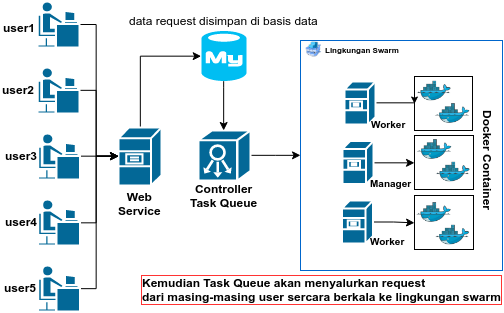
\includegraphics[width=10cm,height=7cm]{Images/C-5/taskqueue.png}
				\caption{Uji fungsionalitas penggunaan \textit{task queue} terhadap \textit{request user}}
				\label{gambartaskqueue}
			\end{figure}
			Uji coba ini dilakukan dengan cara menjalankan \textit{script} yang menggunakan bahasa pemrograman \textit{Python} pada \textit{crontab} yang ada di \textit{linux} dan dijadwalkan setiap 1 menit. Setiap kali pengguna mengirim \textit{request} uji beban melalui web, akan disimpan di basis data \textit{MySQL}. Ketika ada daftar antrian yang ada di basis data \textit{MySQL}, \textit{script} akan mengeksekusi hanya satu \textit{request} yang memiliki \textit{timestamp} paling awal dari beberapa \textit{request} yang lain dan akan dilakukan pengujian terhadap skenario yang dikirim. Setelah pengujian skenario selesai, status akan diubah menjadi \textit{done} dan \textit{script} akan mengeksekusi \textit{request} yang lain satu-persatu. Pada pengujian ini akan dilakukan oleh 5 pengguna yang akan melakukan \textit{request} uji beban. Gambaran pengujian ditunjukkan pada Gambar \ref{gambartaskqueue}.
			
		
		\subsubsection{Uji Fungsionalitas Pengambil Data Uji Beban}
			Uji coba ini dilakukan dengan cara menjalankan \textit{script puppeteer} pada setiap kontainer. \textit{script puppeteer} akan dijalankan ketika ada \textit{request} dari pengguna melalui \textit{web service} yang disediakan sistem. Gambaran pengujian ditunjukkan pada Gambar \ref{ambilhasiluji}.
			\begin{figure}[H]
				\centering
				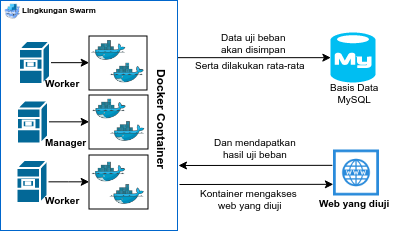
\includegraphics[width=9cm,height=6cm]{Images/C-5/ambilhasiluji.png}
				\caption{Uji fungsionalitas pengambil data uji beban}
				\label{ambilhasiluji}
			\end{figure}
		
		\subsubsection{Uji Fungsionalitas \textit{User} Melihat Hasil Uji Beban}
			Uji coba ini dilakukan dengan mengakses sistem melalui rute \texttt{/hasil}. Pengguna akan mengirimkan \textit{http request} kepada \textit{web service} yang telah disediakan. Rancangan pengujian dan hasil yang diharapkan ditunjukkan pada Tabel \ref{tabelujihasil}.
			\begin{longtable}{|p{0.05\textwidth}|p{0.25\textwidth}|p{0.30\textwidth}|p{0.30\textwidth}|}
				\caption{Skenario uji fungsionalitas \textit{user} melihat hasil uji beban} \label{tabelujihasil} \\ \hline
				\textbf{No} & \textbf{Rute} & \textbf{Uji Coba} & \textbf{Harapan} \\ \hline
				\endhead
				\endfoot
				\endlastfoot
				1 & /hasil/rata-rata & Mengirimkan \textit{request} menuju rute \textit{web service} melalui \textit{browser} & \textit{Request} berhasil diterima oleh \textit{web service}, kemudian \textit{web service} menampilkan hasil perhitungan rata-rata untuk hasil uji beban \\ \hline
				2 & /hasil/error-console & Mengirimkan \textit{request} menuju rute \textit{web service} melalui \textit{browser} & \textit{Request} berhasil diterima oleh \textit{web service}, kemudian \textit{web service} menampilkan daftar \textit{error console} yang terekam pada \textit{browser} \\ \hline
				3 & /hasil/images & Mengirimkan \textit{request} menuju rute \textit{web service} melalui \textit{browser} & \textit{Request} berhasil diterima oleh \textit{web service}, kemudian \textit{web service} menampilkan hasil tangkapan layar web yang diuji pada \textit{browser} \\ \hline
			\end{longtable}
		
	\subsection{Skenario Uji Performa} \label{skenujiperforma}
		Sistem \textit{load generator} dan pengambil data uji beban dibangun pada 3 buah \textit{node host} yang terpasang di lingkungan \textit{swarm}.  Sebelum dilakukan uji performa, dilakukan pemasangan \textit{load generator} yang diinisiasi pada terminal \textit{manager node}, kemudian \textit{manager node} akan mendistribusikan kontainer ke setiap \textit{node host} yang tergabung. Setelah selesai, data dari setiap kontainer akan disimpan di basis data. Uji coba akan dilakukan secara bertahap untuk membuat 500 kontainer, status awal kontainer sebelum diberikan \textit{request} akan \textit{sleep}. Setelah itu uji coba performa dilakukan untuk menguji performa sistem terhadap jumlah \textit{load generator} yang dikirimkan oleh pengguna. Pengujian akan dikirimkan oleh pengguna melalui \textit{web service} yang disediakan sistem. Jumlah \textit{load generator} yang akan diuji mulai dari 100, 200, 300, 400 dan 500. Hasil yang diharapkan dari pengujian performa sistem yaitu \textit{CPU} dan \textit{Memory} yang digunakan pada setiap \textit{node host}. Arsitektur pengujian tertera pada Gambar \ref{ujiperforma}.
		\begin{figure}[H]
			\centering
			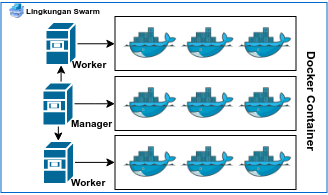
\includegraphics[width=9cm,height=6cm]{Images/C-5/performa.png}
			\caption{Arsitektur uji performa}
			\label{ujiperforma}
		\end{figure}
	
	\section{Hasil Uji Coba dan Evaluasi}
		Berikut dijelaskan hasil uji coba dan evaluasi berdasarkan skenario yang sudah dijelaskan pada bab \ref{skenarioujicoba}.
		
		\subsection{Uji Fungsionalitas}
			Berikut dijelaskan hasil pengujian fungsionalitas pada sistem yang sudah dibangun.
			
			\subsubsection{Uji Fungsionalitas \textit{User} Mengelola Skenario}
				Uji coba ini dilakukan dengan mengakses sistem melalui rute yang telah ditentukan pada Tabel \ref{tabelujiskenario}. Pengguna akan mengirim http request kepada web service yang telah
				disediakan. Hasil uji coba seperti tertera pada Tabel \ref{tabelhasilujiskenario}.
				\begin{longtable}{|p{0.05\textwidth}|p{0.25\textwidth}|p{0.40\textwidth}|p{0.12 \textwidth}|}
					\caption{Skenario uji fungsionalitas \textit{user} mengelola skenario} \label{tabelhasilujiskenario} \\ \hline
					\textbf{No} & \textbf{Rute} & \textbf{Harapan} & \textbf{Hasil} \\ \hline
					\endhead
					\endfoot
					\endlastfoot
					1 & /skenario & \textit{Request} berhasil diterima oleh \textit{web service}, kemudian \textit{web service} mengirimkan umpan balik berupa data skenario dari pengguna yang ditampilkan di \textit{browser} & OK \\ \hline
					2 & /skenario/create & \textit{Request} berhasil diterima oleh \textit{web service} dan halaman untuk membuat skenario ditampilkan di \textit{browser}  & OK \\ \hline
					3 & /skenario & \textit{Web service} berhasil menyimpan data skenario di basis data dan di setiap \textit{node host} dalam bentuk file konfig & OK \\ \hline
					4 & /skenario/\{id\} &\textit{Web service} berhasil menghapus data skenario di basis data dan di setiap \textit{node host} & OK \\ \hline
				\end{longtable}
				
			\subsubsection{Uji Fungsionalitas \textit{User} Mengirim Request Uji Beban}
				Uji coba ini dilakukan dengan mengakses sistem melalui rute yang telah ditentukan pada Tabel \ref{tabelujirequest}. Pengguna akan mengirim http request kepada web service yang telah
				disediakan. Hasil uji coba seperti tertera pada Tabel \ref{tabelhasilujirequest}.
				\begin{longtable}{|p{0.05\textwidth}|p{0.25\textwidth}|p{0.40\textwidth}|p{0.12 \textwidth}|}
					\caption{Skenario uji fungsionalitas \textit{user} mengirim request uji beban} \label{tabelhasilujirequest} \\ \hline
					\textbf{No} & \textbf{Rute} & \textbf{Harapan} & \textbf{Hasil} \\ \hline
					\endhead
					\endfoot
					\endlastfoot
					1 & /worker & \textit{Request} berhasil diterima oleh \textit{web service}, kemudian \textit{web service} menampilkan halaman untuk mengatur jumlah \textit{worker(load generator)} di \textit{browser} & OK \\ \hline
					2 & /worker & \textit{Web service} berhasil menyimpan data \textit{worker} dan membuat antrian \textit{request} di dalam basis data & OK \\ \hline
				\end{longtable}
				
			\subsubsection{Uji Fungsionalitas Penggunaan \textit{Task Queue} Terhadap \textit{Request User}}
				Uji coba ini akan dilakukan oleh 5 user yang melakukan request uji beban melalui \textit{web service} sesuai dengan penjelasan pada bab \ref{quuuueue}. Keterangan hasil uji yang dilakukan bisa dilihat pada Tabel \ref{quuuuueee}.
				\begin{longtable}{|p{0.15\textwidth}|p{0.12\textwidth}|p{0.35\textwidth}|p{0.18\textwidth}|p{0.10\textwidth}|}
					\caption{Hasil penggunaan \textit{task queue} terhadap \textit{request user}} \label{quuuuueee} \\
					\hline
					\textbf{Username} & \textbf{Jumlah} & \textbf{Link} & \textbf{Antrian ke} & \textbf{Hasil} \\ \hline
					\endhead
					\endfoot
					\endlastfoot
					user1 & 100 & https://dev.ppdbsda.net & 1 & OK \\ \hline
					user2 & 200 & https://dev.ppdbsda.net & 2 & OK \\ \hline
					user3 & 300 & https://dev.ppdbsda.net & 3 & OK \\ \hline
					user4 & 400 & https://dev.ppdbsda.net & 4 & OK \\ \hline
					user5 & 500 & https://dev.ppdbsda.net & 5 & OK \\ \hline
				\end{longtable}
				
			\subsubsection{Uji Fungsionalitas Pengambil Data Uji Beban}
				Uji coba ini akan dilakukan oleh \textit{Puppeteer} yang terpasang pada \textit{node host} di lingkungan \textit{swarm}. Skenario pengambil data uji beban sesuai dengan \textit{request task queue} pada Tabel \ref{quuuuueee}. Hasil dari pengujian ini dapat dilihat pada Tabel \ref{dataujibeban}.
				\begin{longtable}{|p{0.15\textwidth}|p{0.15\textwidth}|p{0.12\textwidth}|p{0.15\textwidth}|p{0.18\textwidth}|p{0.13\textwidth}|}
					\caption{Hasil pengambil data uji beban} \label{dataujibeban} \\
					\hline
					\textbf{Username} & \textbf{Response End} & \textbf{CSS Tracing End} & \textbf{DOM Content Loaded} & \textbf{First Meaningful Paint} & \textbf{Load Event End} \\ \hline
					\endhead
					\endfoot
					\endlastfoot
					user1 & 499,17 & 652,53 & 1592,35 & 1636,69 & 2001,26 \\ \hline
					user2 & 503,88 & 655,09 & 1589,95 & 1660,26 & 2010,12 \\ \hline
					user3 & 510,26 & 660,09 & 1567,26 & 1690,82 & 2084,83 \\ \hline
					user4 & 519,98 & 661,13 & 1598,62 & 1699,87 & 2188,10 \\ \hline
					user5 & 523,56 & 665,61 & 1599,40 & 1685,76 & 2190,45 \\ \hline
				\end{longtable}
			
				Selain itu akan didapatkan perhitungan presentase \textit{error} ketika terjadinya \textit{timeout} saat mengakses web yang diuji atau hasil \textit{performance metrics} pada Tabel \ref{dataujibeban} terdapat hasil kurang dari 0 atau minus.
				
			\subsubsection{Uji Fungsionalitas \textit{User} Melihat Hasil Uji Beban}
				Uji coba ini dilakukan dengan mengakses sistem melalui rute yang telah ditentukan pada Tabel \ref{tabelujihasil}. Pengguna akan mengirim \textit{http request} kepada \textit{web service} yang telah
				disediakan. Hasil uji coba seperti tertera pada Tabel \ref{tabelhasilujihasil}.
				\begin{longtable}{|p{0.05\textwidth}|p{0.25\textwidth}|p{0.40\textwidth}|p{0.12 \textwidth}|}
					\caption{Skenario uji fungsionalitas \textit{user} melihat hasil uji beban} \label{tabelhasilujihasil} \\ \hline
					\textbf{No} & \textbf{Rute} & \textbf{Uji Coba} & \textbf{Hasil} \\ \hline
					\endhead
					\endfoot
					\endlastfoot
					1 & /hasil/rata-rata & \textit{Request} berhasil diterima oleh \textit{web service}, kemudian \textit{web service} menampilkan hasil perhitungan rata-rata untuk hasil uji beban & OK \\ \hline
					2 & /hasil/error-console & \textit{Request} berhasil diterima oleh \textit{web service}, kemudian \textit{web service} menampilkan daftar \textit{error console} yang terekam pada \textit{browser} & OK \\ \hline
					3 & /hasil/images & \textit{Request} berhasil diterima oleh \textit{web service}, kemudian \textit{web service} menampilkan hasil tangkapan layar web yang diuji pada \textit{browser} & OK \\ \hline
				\end{longtable}
				

		\subsection{Uji Performa}
			Seperti yang dijelaskan pada bab \ref{skenujiperforma} pengujian performa akan dilakukan pada 3 \textit{node host} yang terpasang di lingkungan \textit{swarm}. Pertama akan dilakukan pembuatan \textit{load generator(worker)} terlebih dahulu, kemudian akan dilakukan uji performa sistem ketika menerima layanan uji beban.
			
			\subsubsection{Uji Pembuatan \textit{Load Generator}}
				Kondisi awal ketersediaan sumberdaya sebelum dilakukan pembuatan \textit{load generator} pada masing-masing \textit{node host} ditunjukkan pada Tabel \ref{suberdayaawalpembuatan}.
				\begin{longtable}{|p{0.05\textwidth}|p{0.25\textwidth}|p{0.14\textwidth}|p{0.17\textwidth}|p{0.14\textwidth}|}
					\caption{Kondisi awal ketersediaan sumberdaya sebelum pembuatan} \label{suberdayaawalpembuatan} \\
					\hline
					\textbf{No} & \textbf{Hostname} & \textbf{CPU} & \textbf{RAM} & \textbf{Storage} \\ \hline
					\endhead
					\endfoot
					\endlastfoot
					1 & CLOUD & 99,70\% & 287M/3.9G & 74/78G \\ \hline
					2 & RAIN & 99,64\% & 256M/3.9G & 74/78G \\ \hline
					3 & STORM & 99,69\% & 255M/3.9G & 74/78G \\ \hline
				\end{longtable}
			
				Setelah dilakukan uji coba untuk membuat kontainer yang akan digunakan sebagai \textit{load generator}, 
				ketersediaan sumberdaya \textit{CPU} dan \textit{RAM} ditunjukkan pada Tabel \ref{suberdayasetpembuatan} serta grafik  kondisi ketersediaan \textit{CPU} setelah pemasangan pada Gambar \ref{pembuatancpu} dan kondisi ketersediaan \textit{RAM} setelah pemasangan pada Gambar \ref{pembuatanram}.
				\begin{longtable}{|p{0.05\textwidth}|p{0.25\textwidth}|p{0.14\textwidth}|p{0.17\textwidth}|}
					\caption{Kondisi ketersediaan sumberdaya setelah pembuatan} \label{suberdayasetpembuatan} \\
					\hline
					\textbf{No} & \textbf{Hostname} & \textbf{CPU} & \textbf{RAM} \\ \hline
					\endhead
					\endfoot
					\endlastfoot
					1 & CLOUD & 97,9\% & 950M/3,9G \\ \hline
					2 & RAIN & 97,9\% & 892M/3,9G \\ \hline
					3 & STORM & 97,8\% & 889M/3,9G \\ \hline
				\end{longtable}
				
				\begin{figure}[H]
					\centering
					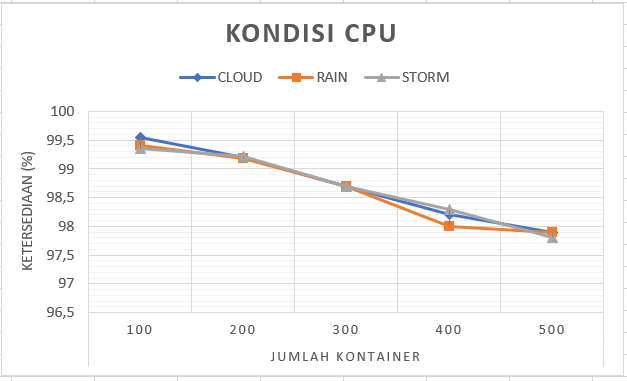
\includegraphics[width=10cm,height=6cm]{Images/C-5/pembuatancpu.PNG}
					\caption{Kondisi ketersediaan sumberdaya \textit{CPU} setelah pembuatan}
					\label{pembuatancpu}
				\end{figure}
				
				\begin{figure}[H]
					\centering
					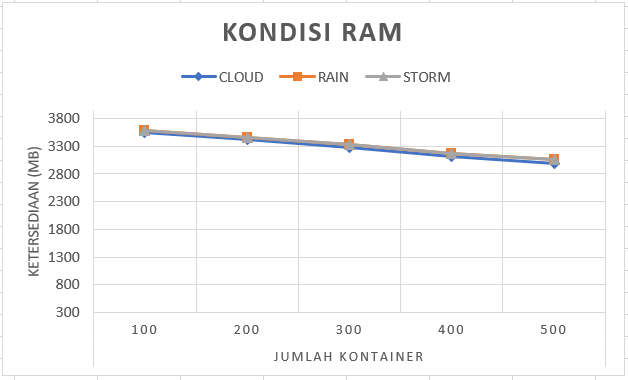
\includegraphics[width=10cm,height=6cm]{Images/C-5/pembuatanram.PNG}
					\caption{Kondisi ketersediaan sumberdaya \textit{RAM} setelah pembuatan}
					\label{pembuatanram}
				\end{figure}
				
				Dari grafik tersebut dapat dilihat kebutuhan sumberdaya \textit{CPU} dan \textit{RAM} tidak mengalami perbedaan yang banyak dan hanya berubah secara \textit{linear}. \textit{CPU} tidak terlalu banyak berubah setelah pembuatan load generator dikarenakan semua \textit{load generator} di atur untuk \textit{sleep} sebelum ada \textit{request} uji beban. Namun ketika pembuatan \textit{load generator} dan pendistribusiannya, tentu saja penggunaan \textit{CPU} bisa sampai 100\% dan untuk penggunaan \textit{RAM} adalah 1,3MB untuk setiap kontainernya. Pada tugas akhir ini, server yang digunakan hanya memiliki spesifikasi 2 \textit{Core CPU}. Adapun masalah-masalah yang dihadapi dalam pengujian ini yaitu ketika membuat \textit{load generator} dengan jumlah diatas 500 secara bersamaan yang akan mengakibatkan \textit{CPU Usage} bisa melebihi kapasitasnya dan hal tersebut akan membuat server \textit{not responding}. Namun untuk penggunaan \textit{RAM} ketika pembuatan masih bisa dikatakan cukup.
				
				Sedangkan hasil distribusi kontainer ke setiap \textit{node host} setelah dilakukan pembuatan \textit{load generator} ditunjukkan pada Tabel \ref{jumlahkontainerpem}.
				\begin{longtable}{|p{0.05\textwidth}|p{0.30\textwidth}|p{0.15\textwidth}|p{0.15\textwidth}|p{0.15\textwidth}|}
					\caption{Hasil distribusi kontainer setelah pembuatan} \label{jumlahkontainerpem} \\
					\hline
					\textbf{No} & \textbf{Jumlah Kontainer} & \textbf{CLOUD} & \textbf{RAIN} & \textbf{STORM} \\ \hline
					\endhead
					\endfoot
					\endlastfoot
					1 & 100 & 34 & 33 & 33 \\ \hline
					2 & 200 & 66 & 67 & 67 \\ \hline
					3 & 300 & 100 & 100 & 100 \\ \hline
					4 & 400 & 132 & 134 & 134 \\ \hline
					5 & 500 & 166 & 167 & 167 \\ \hline
				\end{longtable}
			
				Pendistribusian pada Tabel \ref{jumlahkontainerpem} diatasi oleh manajer pada Docker Swarm dan didistribusikan secara rata ke setiap node host yang tergabung.
			
			\subsubsection{Uji Performa Sistem ketika Menerima Request Layanan Uji Beban}
%				Kondisi awal ketersediaan sumberdaya sebelum ada \textit{request} jumlah \textit{load generator} dari pengguna pada masing-masing \textit{node host} ditunjukkan pada Tabel \ref{suberdayaawalperforma}.
%				\begin{longtable}{|p{0.05\textwidth}|p{0.25\textwidth}|p{0.14\textwidth}|p{0.17\textwidth}|}
%					\caption{Kondisi awal ketersediaan sumberdaya sebelum pembuatan} \label{suberdayaawalperforma} \\
%					\hline
%					\textbf{No} & \textbf{Hostname} & \textbf{CPU} & \textbf{RAM} \\ \hline
%					\endhead
%					\endfoot
%					\endlastfoot
%					1 & CLOUD & 97,9\% & 950M/3,9G \\ \hline
%					2 & RAIN & 97,9\% & 892M/3,9G \\ \hline
%					3 & STORM & 97,8\% & 889M/3,9G \\ \hline
%				\end{longtable}
				
				Pengujian ini dilakukan ketika sistem menerima request layanan uji beban, informasi penggunaan sumberdaya ditunjukkan pada Tabel \ref{sdhasilperforma}, dari tabel tersebut didapatkan grafik penggunaan CPU pada Gambar \ref{performacpu} dan grafik penggunaan RAM pada Gambar \ref{performaram}.
				\begin{longtable}{|p{0.05\textwidth}|p{0.18\textwidth}|p{0.12\textwidth}|p{0.10\textwidth}|p{0.2\textwidth}|}
					\caption{Kondisi penggunaan sumberdaya ketika ada \textit{request}} \label{sdhasilperforma} \\
					\hline
					\textbf{No} & \textbf{Hostname} & \textbf{Jumlah} & \textbf{CPU} & \textbf{RAM} \\ \hline
					\endhead
					\endfoot
					\endlastfoot
					1 & CLOUD & 100 & 39,5\% & 1,1/3,9G \\ \cline{3-5}
					&& 200 & 52\% & 1,2/3,9G \\ \cline{3-5}
					&& 300 & 42,2\% & 1,3/3,9G \\ \cline{3-5}
					&& 400 & 48,7\% & 1,36/3,9G \\ \cline{3-5}
					&& 500 & 50,9\% & 1,39/3,9G \\ \hline
					2 & RAIN & 100 & 36,7\% & 1,02/3,9G \\ \cline{3-5}
					&& 200 & 46\% & 1,18/3,9G \\ \cline{3-5}
					&& 300 & 44,9\% & 1,3/3,9G \\ \cline{3-5}
					&& 400 & 46,8\% & 1,33/3,9G \\ \cline{3-5}
					&& 500 & 49\% & 1,4/3,9G \\ \hline
					3 & STORM & 100 & 38,9\% & 1,05/3,9G \\ \cline{3-5}
					&& 200 & 23\% & 1,12/3,9G \\ \cline{3-5}
					&& 300 & 40,2\% & 1,19/3,9G \\ \cline{3-5}
					&& 400 & 44,9\% & 1,38/3,9G \\ \cline{3-5}
					&& 500 & 49,6\% & 1,45/3,9G \\ \hline
				\end{longtable}
			
				\begin{figure}[H]
					\centering
					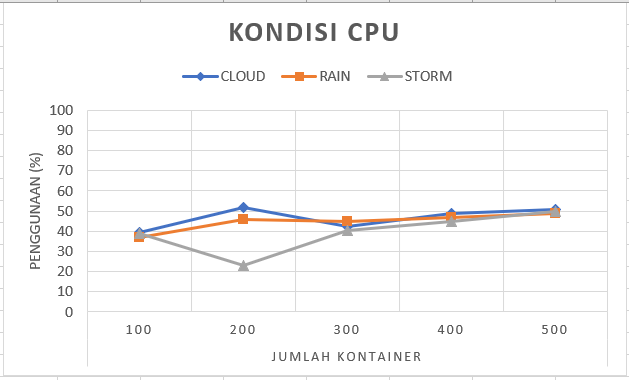
\includegraphics[width=10cm,height=5.5cm]{Images/C-5/performacpu.PNG}
					\caption{Kondisi penggunaan sumberdaya \textit{CPU} ketika ada \textit{request}}
					\label{performacpu}
				\end{figure}
			
				Dilihat dari grafik pada Gambar \ref{performacpu}, penggunaan \textit{CPU} mengalami perubahan secara \textit{linear} yaitu semakin banyak \textit{request} uji beban akan semakin tinggi, namun pada saat pengujian ketika jumlah \textit{load generator} 200, terjadi anomali pada ketersediaan sumberdaya, hal tersebut dikarenakan urutan kontainer id yang disimpan pada basis data tidak berimbang untuk nomor urut dari 1 sampai 200, sehingga pada \textit{node host} CLOUD dan RAIN memiliki jumlah \textit{load generator} yang harus dijalankan jauh lebih banyak dari pada \textit{node host} STORM, sehingga mengakibatkan tenjadinya anomali penggunaan \textit{CPU} pada \textit{node host} STORM.
				
				\begin{figure}[H]
					\centering
					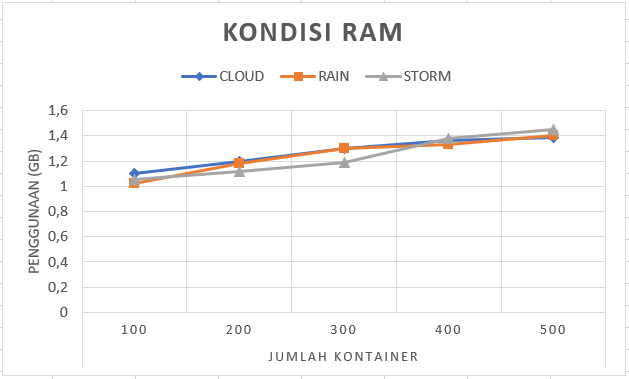
\includegraphics[width=10cm,height=5.5cm]{Images/C-5/performaram.PNG}
					\caption{Kondisi penggunaan sumberdaya \textit{RAM} ketika ada \textit{request}}
					\label{performaram}
				\end{figure}
				
				Sedangkan untuk penggunaan \textit{RAM} pada Gambar \ref{performaram}, perubahannya secara linear saja, dikarenakan memang adanya pembatasan berjalannya proses secara bersama dalam setiap waktunya, karena \textit{Chrome} yang dijalankan akan memerlukan sumberdaya yang banyak. Jika tidak dibatasi, dapat mengakibatkan penggunaan \textit{CPU} dan \textit{RAM} akan melebihi kapasitas dan mengakibatkan server menjadi \textit{not responding}. Dapat disimpulkan juga dalam melakukan uji beban menggunakan \textit{Headless Chrome} akan membutuhkan banyak sumberdaya \textit{CPU} dan \textit{RAM}, sedangkan untuk penggunaan \textit{Docker} tidak memerlukan sumberdaya sebanyak \textit{Headless Chrome}.
				